\section{Experimental Setup}

\subsection{Environment}

The N-Back experiment was conducted at the Language Acquisition and Language Processing Lab at the Department of Language and Literature at NTNU. This lab hosts advanced equipment and facilities for research in experimental linguistics, psycholinguistics, and neurolinguistics. In addition to two \acrshort{eeg} systems and an fNIRS system, they offer a variety of advanced research-grade eye trackers, one of which will be detailed in the subsection below. 

The eye-tracking environment was fully enclosed to avoid outside disturbance during task operation. It was moderately lit to avoid interference in pupil diameter from the \acrshort{plr}. The screen which displayed the task stimulus was placed at a constant 65cm from the subject, ensuring minimal interference from the \acrshort{pnr} as well. The reason for such considerations were explained in section \ref{sec:bt/cognitive_impacts/plr_pnr}. 

Recording sessions were limited to approximately five minutes (three N-Back blocks, each lasting about one and a half minutes), with at least two minutes of relaxation between sessions. This was done to mitigate the effects of fatigue on task performance. Additionally, since the author of this thesis was also the experimental subject, he was encouraged to be fully engaged in every task to ensure optimal data quality.

\subsection{Hardware}

The hardware used to record eye-tracking data was a Tobii Pro Spectrum, in a setup shown in image \ref{fig:impl_hardware_setup}. This tracker has the advantage of having a permanently mounted stimulus screen. This setup minimizes error from poorly calibrated manual screen configurations, which is often the case with other models. Said stimulus screen was 23.8-inches wide and LED-backlit, with an aspect ratio of 16:9 and 1080p resolution.

\begin{figure}[h]
    \centering
    \includegraphics[width=0.8\textwidth]{figures/impl_hardware_setup.png}
    \caption{Hardware setup of a Tobii Pro Spectrum in the Language Acquisition and Language Processing Lab.}
    \label{fig:impl_hardware_setup}
\end{figure}

The eye-tracker itself was mounted directly beneath the screen. It uses the pupil- and corneal reflection method detailed in section \ref{sec:bt/ET_tech} to capture data in a non-intrusive manner. Its remote capabilities allow for free head movement within a 34cm x 26cm (width x height) track box, at 60cm to 80cm from the stimulus screen. Two cameras that capture stereo images of both eyes combined with nine infrared illuminators provide accurate estimations of on-screen gaze, 3D head position, and pupil diameter. All this data is streamed at up to 1200 samples per second, allowing for the capture of high-fidelity eye movements, tiny deviations in pupil diameter, and high-frequency oscillatory eye movements such as microsaccades. 

On-screen coordinates as output from the eye-tracker are depicted in figure \ref{fig:impl_output}. They are given in floating-point values from (0.0, 0.0) in the top-left corner to (1.0, 1.0) in the bottom-right corner. Upon installation, between subjects and otherwise, as often as possible, a calibration is required to get accurate gaze estimations.

\begin{figure}[h]
    \centering
    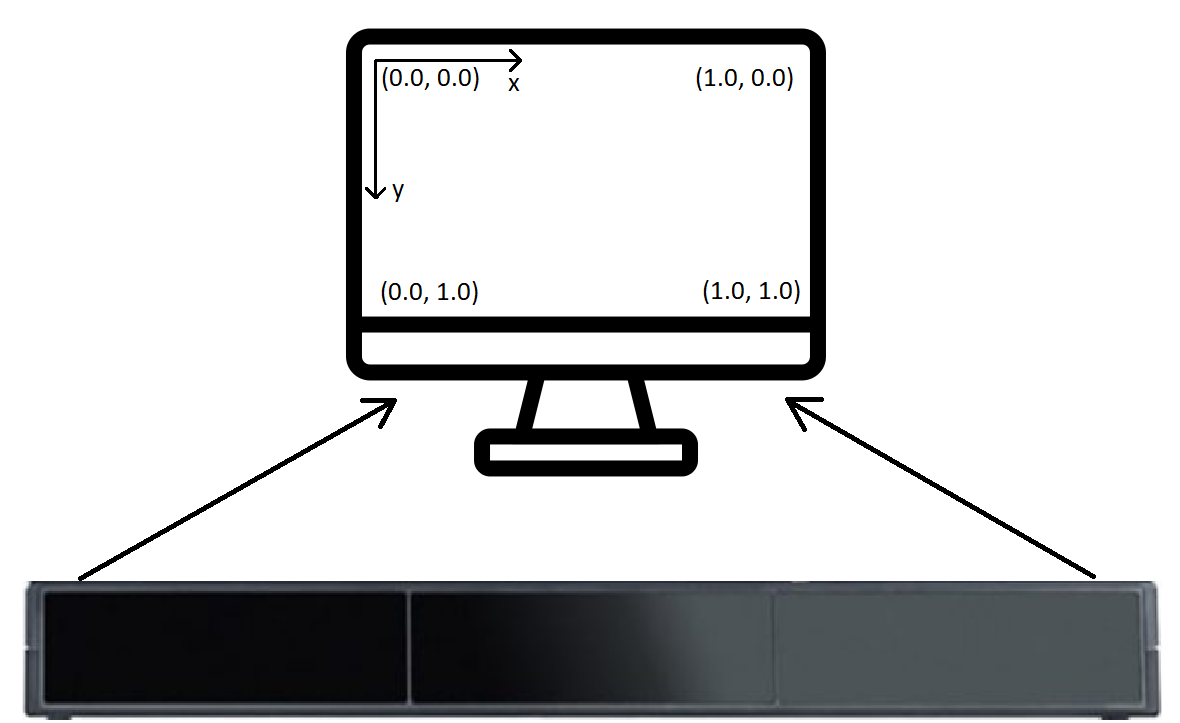
\includegraphics[width=0.8\textwidth]{figures/impl_output.png}
    \caption{Schematic representation of the coordinate system in which on-screen gaze data is presented by the Tobii Pro Spectrum.}
    \label{fig:impl_output}
\end{figure}